\documentclass[xetex,mathserif,serif]{beamer}

\usepackage{xunicode}
\usepackage{xltxtra}
\usepackage{color}
\usepackage{url}
\usepackage{listings}
\usepackage{fontspec}
\usepackage{geometry}
\usepackage{lastpage}
\usepackage{fancyhdr}
\usepackage{amsmath}
\usepackage{amsthm}
\usepackage{amssymb}
\usepackage{blkarray}
\usepackage{multicol}
\usepackage{relsize}

\definecolor{solarized@base03}{HTML}{002B36}
\definecolor{solarized@base02}{HTML}{073642}
\definecolor{solarized@base01}{HTML}{586e75}
\definecolor{solarized@base00}{HTML}{657b83}
\definecolor{solarized@base0}{HTML}{839496}
\definecolor{solarized@base1}{HTML}{93a1a1}
\definecolor{solarized@base2}{HTML}{EEE8D5}
\definecolor{solarized@base3}{HTML}{FDF6E3}
\definecolor{solarized@yellow}{HTML}{B58900}
\definecolor{solarized@orange}{HTML}{CB4B16}
\definecolor{solarized@red}{HTML}{DC322F}
\definecolor{solarized@magenta}{HTML}{D33682}
\definecolor{solarized@violet}{HTML}{6C71C4}
\definecolor{solarized@blue}{HTML}{268BD2}
\definecolor{solarized@cyan}{HTML}{2AA198}
\definecolor{solarized@green}{HTML}{859900}
\definecolor{yaleblue}{HTML}{0E4C92}

\newcommand{\yellow}[1]{\textcolor{solarized@yellow}{#1}}
\newcommand{\orange}[1]{\textcolor{solarized@orange}{#1}}
\newcommand{\red}[1]{\textcolor{solarized@red}{#1}}
\newcommand{\magenta}[1]{\textcolor{solarized@magenta}{#1}}
\newcommand{\violet}[1]{\textcolor{solarized@violet}{#1}}
\newcommand{\blue}[1]{\textcolor{solarized@blue}{#1}}
\newcommand{\cyan}[1]{\textcolor{solarized@cyan}{#1}}
\newcommand{\green}[1]{\textcolor{solarized@green}{#1}}
\newcommand{\yblue}[1]{\textcolor{yaleblue}{#1}}

\setbeamertemplate{navigation symbols}{}
% \setbeamerfont{title}{family=\old}
% \setbeamerfont{author}{family=\tfont}%
% \setbeamerfont{frametitle}{family=\oldA}
% \setbeamerfont{date}{family=\dfont}

% \addtobeamertemplate{navigation symbols}{}{%
%     \usebeamerfont{footline}%
%     \usebeamercolor[fg]{footline}%
%     \hspace{1em}%
%     \insertframenumber/\inserttotalframenumber
% }

\setbeamertemplate{footline}[text line]{%
  \parbox{0.99\linewidth}{
    \normalsize\vspace*{-24pt}\hfill{\color{solarized@base00}\insertframenumber/\inserttotalframenumber}
  }
}


\setbeamertemplate{itemize items}{--}
\setbeamercolor*{item}{fg=black}

\defaultfontfeatures{Mapping=tex-text}
\hypersetup{pdfstartview={FitH}}

\newcommand{\old}[1]{\fontspec[Alternate=1,Ligatures={Common}]{Hoefler Text}\fontsize{18pt}{30pt}\selectfont #1}%
\newcommand{\oldA}[1]{\fontspec[Alternate=1,Ligatures={Common, Rare}]{Hoefler Text}\fontsize{12pt}{15pt}\selectfont #1}%
\newcommand{\oldB}[1]{\fontspec[Ligatures={Common}]{Didot}\fontsize{12pt}{15pt}\color{solarized@base02}\selectfont #1}%
\newcommand{\tfont}[1]{\fontspec[Alternate=1,Ligatures={Common}]{Hoefler Text}\fontsize{12pt}{20pt}\selectfont #1}%
\newcommand{\dfont}[1]{\fontspec[Ligatures={Common}]{Didot}\fontsize{12pt}{12pt}\selectfont #1}%

% \newcommand{\minimize}{\mathop{\mathrm{minimize}}}
\newcommand{\argmin}{\mathop{\mathrm{arg\,min}}}
\newcommand{\argmax}{\mathop{\mathrm{arg\,max}}}
\newcommand{\st}{\mathop{\mathrm{subject\,\,to}}}

\newcommand\independent{\protect\mathpalette{\protect\independenT}{\perp}}
\def\independenT#1#2{\mathrel{\rlap{$#1#2$}\mkern2mu{#1#2}}}

\setlength{\parindent}{0pt}
\setlength{\parskip}{12pt}

\setromanfont [Ligatures={Common}, Numbers={OldStyle}, Variant=01,
 BoldFont={LinLibertine_RB.otf},
 ItalicFont={LinLibertine_RI.otf},
 BoldItalicFont={LinLibertine_RBI.otf}
 ]{LinLibertine_R.otf}



\usepackage{sty/personalmacros}
\usepackage{sty/personalslides}

\begin{document}
%%%%%%%%%%%%%%%%%%%%%%%%%%%%%%%%%%%%%%%%%%%%%%%%%%%%%%%%%%%%%%%%%%%%%%%%%%%%%%%
\begin{frame}[fragile] \frametitle{}
\vfill
{
    \color{yaleblue}
    \fontsize{0.5cm}{0cm}\selectfont
    Paper Presentation: \\
}
\vspace{0.5cm}
Hofree, \textit{et al.}\\
\vspace{0.1cm}
{
    \fontsize{0.7cm}{0cm}\selectfont
    Network-based stratification of tumor mutations.\\
}
\vspace{0.1cm}
\textit{Nature Methods.} (2013).\\

\hfill

\vspace{2cm}
\begin{minipage}{1.0\textwidth}\raggedleft
    \color{yaleblue}
    Addison Hu   \\
    CB\&B 555\\
    8 December 2016
\end{minipage}
\end{frame}
%%%%%%%%%%%%%%%%%%%%%%%%%%%%%%%%%%%%%%%%%%%%%%%%%%%%%%%%%%%%%%%%%%%%%%%%%%%%%%%
%
%%%%%%%%%%%%%%%%%%%%%%%%%%%%%%%%%%%%%%%%%%%%%%%%%%%%%%%%%%%%%%%%%%%%%%%%%%%%%%%
\begin{frame}[fragile] \frametitle{}
    \slideheader{Biological Motivation: Cancer Subtype Discovery}
    \begin{itemize}
        \item Many forms of cancer consist of multiple subtypes with different
            causes and clinical outcomes.
        \item Identification of these subtypes are of key interest.
        \item In \textit{tumor stratification},
            a population of tumors is divided into meaningful subtypes
            based on similarity of molecular profiles.
        \item Past work in this regard has focused on mRNA expression data;
            shortcomings include RNA sample quality and  lack of
            reproducibility between biological replicates.
    \end{itemize}
\end{frame}
%%%%%%%%%%%%%%%%%%%%%%%%%%%%%%%%%%%%%%%%%%%%%%%%%%%%%%%%%%%%%%%%%%%%%%%%%%%%%%%
\begin{frame}[fragile] \frametitle{}
    \slideheader{Background: Somatic Mutation Profile}
    \begin{itemize}
        \item High-throughput sequencing is used to identify mutations that
            have become enriched in the tumor cell population.
        \item Assumption: this set of mutations contain the causal drivers
            of tumor progression; therefore, similarities and differences in
            mutations across patients can guide tumor stratification.
        \item Problem: Somatic mutation profiles are highly sparse; typically
            fewer than 100 mutated bases are found in the entire exome.
    \end{itemize}
    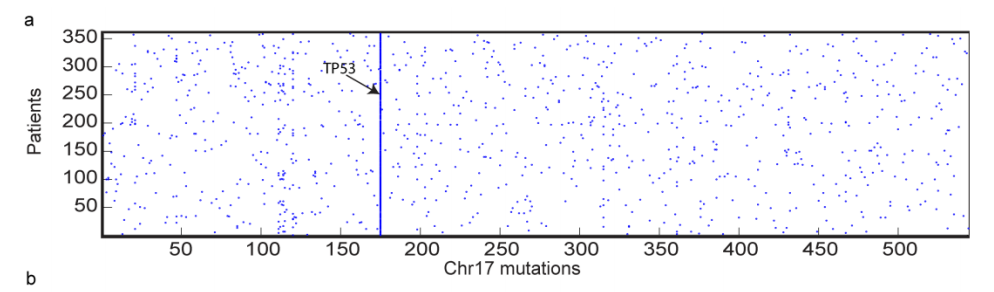
\includegraphics[scale=0.3]{img/suppfig1.png}
\end{frame}
%%%%%%%%%%%%%%%%%%%%%%%%%%%%%%%%%%%%%%%%%%%%%%%%%%%%%%%%%%%%%%%%%%%%%%%%%%%%%%%
\begin{frame}[fragile] \frametitle{}
    \slideheader{Hypothesis: Use Gene Network Information}
    \begin{itemize}
        \item Authors sought to integrate somatic tumor genomes with gene
            interaction networks.
        \item Assumption: Although two tumors may not have any mutations in
            common, they may share the networks affected by these mutations.
        \item Idea: Use network knowledge to cluster somatic mutation profiles
            into tumor subtypes that both provide biological insight and are
            tied to clinical outcomes (e.g., patient survival time, emergence
            of drug resistance).
    \end{itemize}
\end{frame}
%%%%%%%%%%%%%%%%%%%%%%%%%%%%%%%%%%%%%%%%%%%%%%%%%%%%%%%%%%%%%%%%%%%%%%%%%%%%%%%
\begin{frame}[fragile] \frametitle{}
    \slideheader{Data}
    \begin{itemize}
        \item Data obtained from the Cancer Genome Atlas
        \item Techniques demonstrated with ovarian, uterine, and lung cancer
            cohorts
        \item Somatic mutations for each patient are represented as a series
            of binary states $\{0, 1\}$ on genes; a $1$ denotes that a mutation
            has occurred for a gene relative to the germ line.
        \item Each patient's mutation profile is projected onto a human gene
            interaction network obtained from public databases (e.g., 
            STRING\footnote{
                Szklarczyk, D. \textit{et al.} The STRING database in 2011:
                functional interaction networks of proteins, globally
                integrated and scored. \textit{Nucleic Acids Res.} (2011).},
            Pathway Commons\footnote{
                Cerami, E.G. \textit{et al.}
                Pathway Commons, a web resource for biological pathway data.
                \textit{Nucleic Acids Res.} (2011).\vspace{0.2cm}}).
    \end{itemize}
\end{frame}
%%%%%%%%%%%%%%%%%%%%%%%%%%%%%%%%%%%%%%%%%%%%%%%%%%%%%%%%%%%%%%%%%%%%%%%%%%%%%%%
%
%%%%%%%%%%%%%%%%%%%%%%%%%%%%%%%%%%%%%%%%%%%%%%%%%%%%%%%%%%%%%%%%%%%%%%%%%%%%%%%
%%%%%%%%%%%%%%%%%%%%%%%%%%%%%%%%%%%%%%%%%%%%%%%%%%%%%%%%%%%%%%%%%%%%%%%%%%%%%%%
\begin{frame}[fragile] \frametitle{}
    \slideheader{Network-based Stratification: Overview}
    \begin{center}
        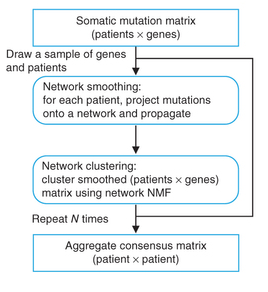
\includegraphics[scale=0.65]{img/overview.png}
    \end{center}
    \iffalse
    \begin{enumerate}
        \item For each patient, project mutations onto a gene interaction
            network.
        \item Smooth the network of binary states using a random walk.
        \item For the matrix of `network-smoothed' patient profiles, perform
            clustering via network-regularized non-negative matrix
            factorization (many times, with subsampling).
        \item Use consensus clustering on the resultant clusters to promote
            robust cluster assignments.
    \end{enumerate}
    \fi
\end{frame}
%%%%%%%%%%%%%%%%%%%%%%%%%%%%%%%%%%%%%%%%%%%%%%%%%%%%%%%%%%%%%%%%%%%%%%%%%%%%%%%
\begin{frame}[fragile] \frametitle{}
    \slideheader{Network smoothing} \\
    \vspace{0.5cm}
    After mapping the patient mutation profile onto a molecular network, the
    state of each gene is in $\{0, 1\}$.    \\
    \vspace{0.2cm}
    Network propagation smooths the mutation signal across the network by
    simulating a random walk on the network:
    $$
    F_{t+1} = \alpha F_t A + (1 - \alpha) F_0
    $$
    where $F_0$ is a patient-by-gene matrix, $A$ is a row-normalized
    adjacency matrix of the gene interaction network, and $\alpha$ is a
    tuning parameter that controls the distance that a mutation signal is
    allowed to diffuse through the network. \\
    \vspace{0.2cm}
    Because each row of $F$ corresponds to a patient, we are essentially
    running a random walk for each patient.
\end{frame}
%%%%%%%%%%%%%%%%%%%%%%%%%%%%%%%%%%%%%%%%%%%%%%%%%%%%%%%%%%%%%%%%%%%%%%%%%%%%%%%
\begin{frame}[fragile] \frametitle{}
    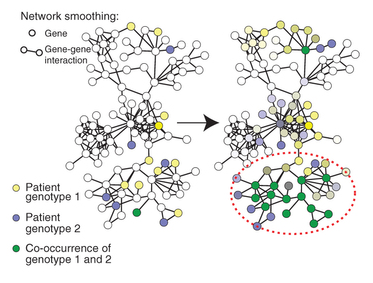
\includegraphics[width=\textwidth]{img/network_smoothing.png}
\end{frame}
%%%%%%%%%%%%%%%%%%%%%%%%%%%%%%%%%%%%%%%%%%%%%%%%%%%%%%%%%%%%%%%%%%%%%%%%%%%%%%%
\iffalse
\begin{frame}[fragile] \frametitle{}
    \slideheader{Non-Negative Matrix Factorization} \\
    \vspace{0.5cm}
    Non-negative matrix factorization is an unsupervised technique in which
    a data matrix $F \in \mathbf{R}_+^{n\times d}$ is decomposed into matrices
    $W\in\mathbf{R}_+^{n\times d}, H\in\mathbf{R}_+^{d\times k}$.   \\
    \pause
    \vspace{0.2cm}
    This decomposition can be solved as an optimization problem with respect
    to the Frobenius norm:
    \begin{align*}
        \minimize{\norm{F - WH}_F^2}{W, H}{W \in \RR_+^{n\times d},
        H \in \RR_+^{d\times k}}
    \end{align*}
    \pause
    NMF has a nice clustering interpretation in which $H$ can be thought of
    as a set of centers (or basis vectors), and $W$ as a matrix of
    weights (for each observation).
\end{frame}
\fi
%%%%%%%%%%%%%%%%%%%%%%%%%%%%%%%%%%%%%%%%%%%%%%%%%%%%%%%%%%%%%%%%%%%%%%%%%%%%%%%
\begin{frame}[fragile] \frametitle{}
    \slideheader{Network-Regularized NMF}   \\
    \vspace{0.5cm}
    Non-negative matrix factorization is an unsupervised technique in which
    a data matrix $F \in \mathbf{R}_+^{n\times d}$ is decomposed into matrices
    $W\in\mathbf{R}_+^{n\times k}, H\in\mathbf{R}_+^{k\times d}$
    \begin{align*}
        \minimize{
            \norm{F - WH}_F^2 + \tr(W^T K W)
        }{W, H}{
            W \in \RR_+^{n\times k},
            H \in \RR_+^{k\times d}
        }
    \end{align*}
    Here, a regularization term derived from the adjacency matrix
    \iffalse
    \footnote{
        $K$ is the adjacency matrix of a nearest neighbors graph derived from
        the graph Laplacian of an influence distance matrix, which in turn is
        derived from the original network.
        \vspace{0.2cm}
    }
    \fi
    is used to constrain the basis vectors in $W$ to respect the
    local network neighborhoods.\footnote{
        Deng, \textit{et al.} Non-negative Matrix Factorization on Manifold.
        in \textit{8th IEEE Int. Conf. Data Mining} (IEEE, 2008).
        \vspace{0.2cm}
    }\\
    \vspace{0.2cm}
    The authors chose $k=12$ subtypes.
\end{frame}
%%%%%%%%%%%%%%%%%%%%%%%%%%%%%%%%%%%%%%%%%%%%%%%%%%%%%%%%%%%%%%%%%%%%%%%%%%%%%%%
\begin{frame}[fragile] \frametitle{}
    %% http://ottechblog.com/wp-content/uploads/2015/01/Screen-Shot-2015-01-04-at-11.01.05-PM.png
    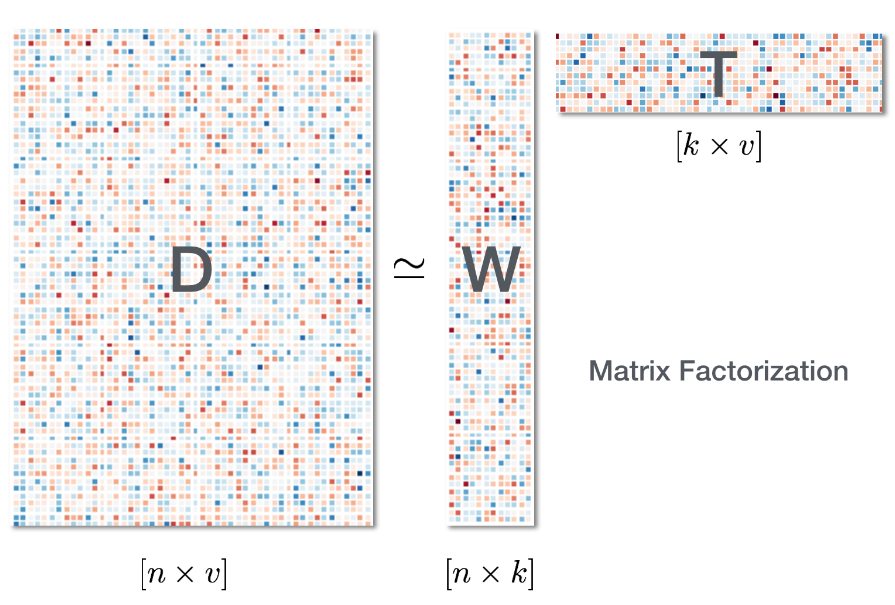
\includegraphics[width=\textwidth]{img/nmf.png}
\end{frame}
%%%%%%%%%%%%%%%%%%%%%%%%%%%%%%%%%%%%%%%%%%%%%%%%%%%%%%%%%%%%%%%%%%%%%%%%%%%%%%%
\iffalse
\begin{frame}[fragile] \frametitle{}
    \slideheader{Consensus Clustering}
    \begin{itemize}
        \item Refers to reconciliation of several distinct clusterings for a
            single dataset (e.g., clusterings from different sources, or
            from numerous applications of a randomized algorithm).
        \item Unsupervised analog to ensemble learning (e.g., random forests
            for decision trees) in supervised learning.
    \end{itemize}
\end{frame}
\fi
%%%%%%%%%%%%%%%%%%%%%%%%%%%%%%%%%%%%%%%%%%%%%%%%%%%%%%%%%%%%%%%%%%%%%%%%%%%%%%%
\begin{frame}[fragile] \frametitle{}
    \slideheader{Consensus Clustering}
    \begin{itemize}
        \item Authors performed network-regularized NMF 1,000 times on
            subsamples\footnote{
                 For each subsample, take 80\% of the patients and 80\% of the
                 mutated genes at random without replacement 
                 \vspace{0.2cm}
             } of the dataset, then turned the resultant clustering
            outcomes into a co-clustering matrix of patients.
        \item The co-clustering matrix records the frequency that each
            patient pair shared membership in the same subtype over across
            all clustering iterations.
        \item Consensus clusters were then derived from this matrix through
            techniques such as average linkage hierarchical clustering.
    \end{itemize}
\end{frame}
%%%%%%%%%%%%%%%%%%%%%%%%%%%%%%%%%%%%%%%%%%%%%%%%%%%%%%%%%%%%%%%%%%%%%%%%%%%%%%%
\begin{frame}[fragile] \frametitle{}
    \sectionslide{Results \& Validation}
\end{frame}
%%%%%%%%%%%%%%%%%%%%%%%%%%%%%%%%%%%%%%%%%%%%%%%%%%%%%%%%%%%%%%%%%%%%%%%%%%%%%%%
\iffalse
\begin{frame}[fragile] \frametitle{}
    \slideheader{Technique Performance on Simulated Data}
    \begin{itemize}
        \item Somatic mutation data simulated using structure of the TCGA
            ovarian tumor mutation data and the STRING gene interaction network.
        \item Improvement in cancer subtype recovery compared to techniques not
            based on network knowledge.
        \item Performance of technique depended on NMF clustering; hierarchical
            clustering led to poorer results.
        \item Network-based stratification outperforms standard consensus
            clustering when there is less likely to be substantial overlap
            in mutations among patients of the same subtype (e.g., lower
            mutation frequencies, larger network modules).
    \end{itemize}
\end{frame}
\fi
%%%%%%%%%%%%%%%%%%%%%%%%%%%%%%%%%%%%%%%%%%%%%%%%%%%%%%%%%%%%%%%%%%%%%%%%%%%%%%%
\begin{frame}[fragile] \frametitle{}
    \slideheader{Performance on Tumor Mutation Data}
    \begin{itemize}
        \item The authors used NBS to stratify patients profiled by TCGA
            (Cancer Genome Atlas) full-exome sequencing for uterine,
            ovarian, and lung cancers.
        \item In each of the three cancers, NBS resulted in robust subtype
            structure; standard consensus clustering (not based on network
            structure) was unable to stratify the patient cohort.
        \item Results held for all three gene networks used.\footnote{
                STRING, HumanNet, PathwayCommons.
                \vspace{0.2cm}
            }
    \end{itemize}
\end{frame}
%%%%%%%%%%%%%%%%%%%%%%%%%%%%%%%%%%%%%%%%%%%%%%%%%%%%%%%%%%%%%%%%%%%%%%%%%%%%%%%
\begin{frame}[fragile] \frametitle{}
    \slideheader{NBS-Identified Subtype \& Observed Clinical Data}
    \begin{itemize}
        \item \textbf{Uterine cancer}: identified subtypes closely associated
            with the recorded subtype on a histological basis (microscopic
            analysis)
        \item \textbf{Ovarian \& Lung cancers}: identified subtypes were
            significant predictors of patient survival time, independently of
            clinical covariates (e.g., tumor stage, age, mutation rate, etc.)
        \item Permuting the mapping between mutated genes and the network
            yielded poorer performance of network-based stratification.
        \item Predictions based on NBS-derived subtypes were competitive
            with those derived from other TCGA data types, e.g., copy-number
            variation, methylation, mRNA expression, microRNA expression,
            protein profiles.
    \end{itemize}
\end{frame}
%%%%%%%%%%%%%%%%%%%%%%%%%%%%%%%%%%%%%%%%%%%%%%%%%%%%%%%%%%%%%%%%%%%%%%%%%%%%%%%
\begin{frame}[fragile] \frametitle{}
    \slideheader{Network Region Identification by Subtype}  
    \\ \vspace{0.5cm}
    The authors also sought to identify regions of the gene network most
    responsible for discriminating the somatic mutation profiles of tumors
    of different subtypes, focusing on ovarian cancer.
    \begin{itemize}
        \item For each subtype, the authors identified the genes for which the
            network-smoothed mutation state differed significantly for patients
            of that subtype versus the others.
        \item This partitioning of genes was projected onto the HumanNet network.
    \end{itemize}
\end{frame}
%%%%%%%%%%%%%%%%%%%%%%%%%%%%%%%%%%%%%%%%%%%%%%%%%%%%%%%%%%%%%%%%%%%%%%%%%%%%%%%
\begin{frame}[fragile] \frametitle{}
    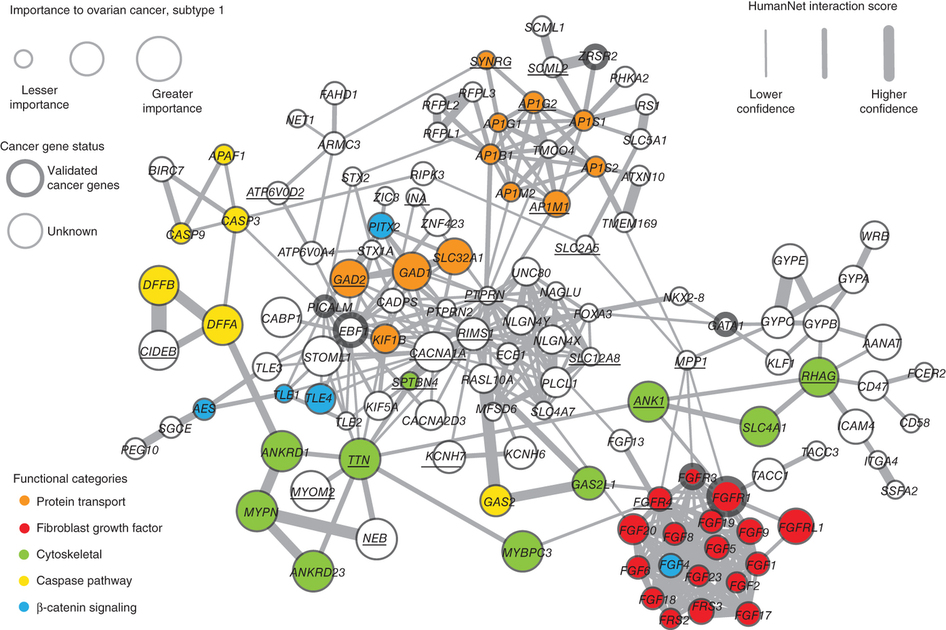
\includegraphics[width=\textwidth]{img/network_subtype.jpg}
\end{frame}
%%%%%%%%%%%%%%%%%%%%%%%%%%%%%%%%%%%%%%%%%%%%%%%%%%%%%%%%%%%%%%%%%%%%%%%%%%%%%%%
\begin{frame}[fragile] \frametitle{}
    \slideheader{Conclusion}
    \begin{itemize}
        \item Incorporating network knowledge improves tumor subtype
            stratification techniques.
        \item Performance of technique was measured against subtype
            identifiability and clinical outcome predictability for uterine,
            ovarian, and lung cancers.
        \item Identifiability depended on network structure; permuting the
            mapping between mutations and the network resulted in poorer
            performance.
    \end{itemize}
\end{frame}
%%%%%%%%%%%%%%%%%%%%%%%%%%%%%%%%%%%%%%%%%%%%%%%%%%%%%%%%%%%%%%%%%%%%%%%%%%%%%%%
\end{document}

